\clearpage
\chapter{Introduction}
\label{ch:intro}

As robots continue to become more integrated into our daily lives, researchers are working to improve human-robot interaction. Gesture recognition technology has emerged as a key tool for enabling more natural interactions with robots, replacing traditional human-machine interfaces like keyboards, mice, and joysticks. This application can be a good intervention for people with disabilities. By using hand gestures, they can more easily interact with virtual environments, robotics, home automation, clinical operations, game controls, desktop/tablet applications, delivery services, sign language, and more. 
Drones are remotely controlled robots can be operated via a remote control device or smartphone. They're a popular tool in many of these applications, often used for sports event coverage, aerial photography, and emergency response. Developing automatic systems that can recognize hand gestures would greatly improve the ability to interact with drones intuitively.
\\ Our goal is to create a real-time hand gesture recognition system for human-drone interaction. In this project, we have achieved touchless interaction between the drone and our hands. We utilized machine learning technology, specifically MediaPipe, for hand tracking and developed a gesture recognition model that underwent rigorous training and testing. The process involves five steps: 
\begin{enumerate}[label=\Roman*.]
	\item Drone capturing an image
	\item Image processing via OpenCV
	\item Gesture recognition
	\item Gesture - command conversion
	\item Command execution
	
\end{enumerate}
Gesture recognition is used in various sectors, including smart home automation and the medical field. It mainly focuses on human-machine interaction. The system receives input images from a drone camera connected to the device. The main goal of this project is to propose a real-time system with high accuracy. In summary, the project demonstrates how we can control a drone in an entertaining and educational way while highlighting the potential of gesture recognition technology in various industries and applications.
\begin{figure}
	\centering
	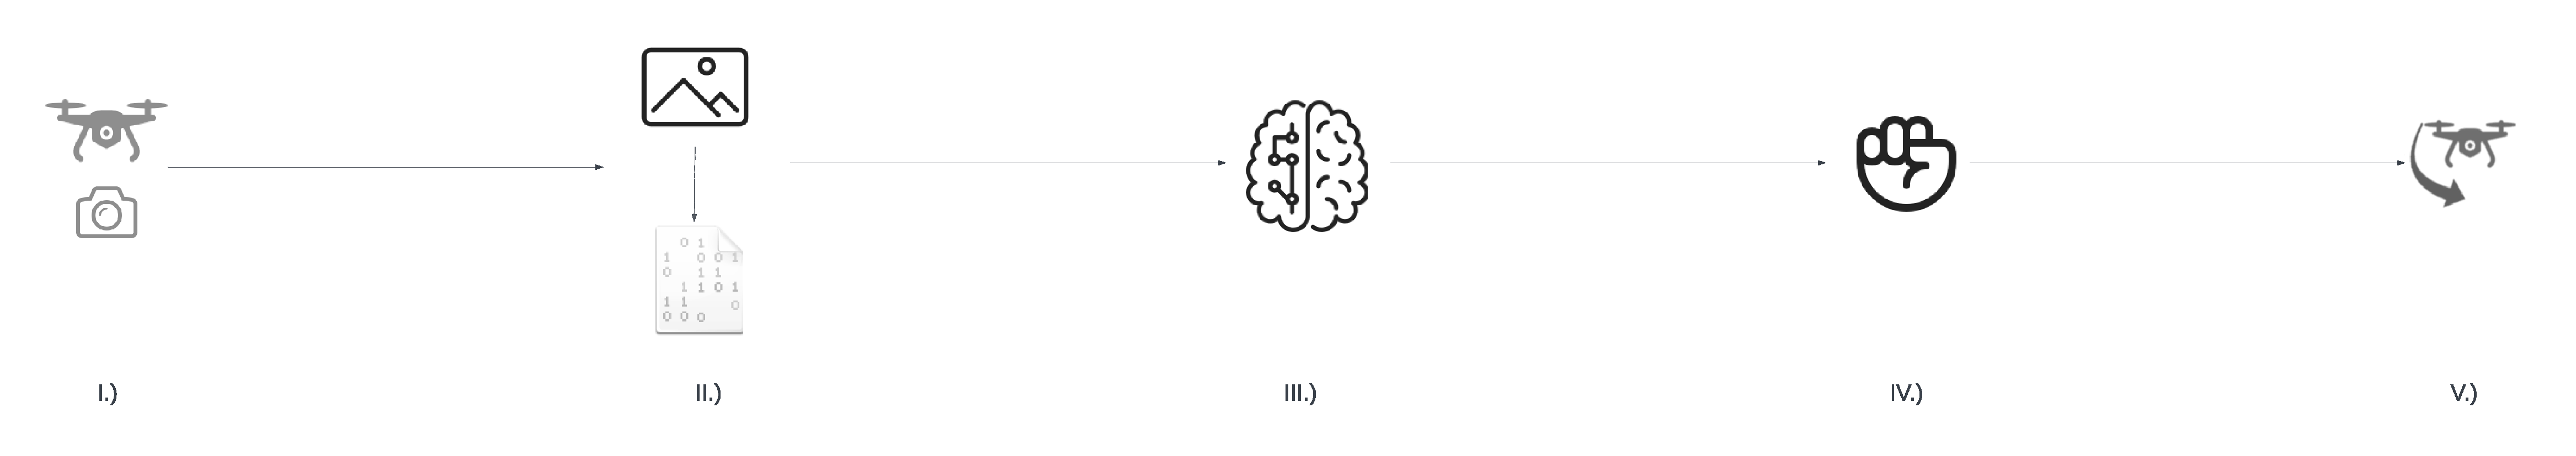
\includegraphics[width = \textwidth]{images/steps.pdf}
	\caption{Steps of the process}
	\label{fig:conclusion}
\end{figure}
